\chapter{Drupal commerce}

\section{Installing the Commerce module(s)}

Drupal commerce is a set of Drupal modules which add web store functionality to our site. The project is maintained by the commerce guys (\url{https://commerceguys.com/}), it is free and opens source (\url{https://github.com/commerceguys}). Since no official version of Drupal commerce has been released for Drupal 8, we are going to use the development version. This could lead to some unexpected problems but as you know, developers like lining on the edge.
The installation instructions can be found here: \url{https://github.com/commerceguys/commerce}. To install the modules we are going to use drush, which stands for Drupal SHell. Drush is a command line tool which makes some tasks a lot easier. To open a Drush console you can click the console window button in the Acquia Dev Desktop (Figure \ref{fig:console_window_button}).

\begin{figure}[H]
	\centering
	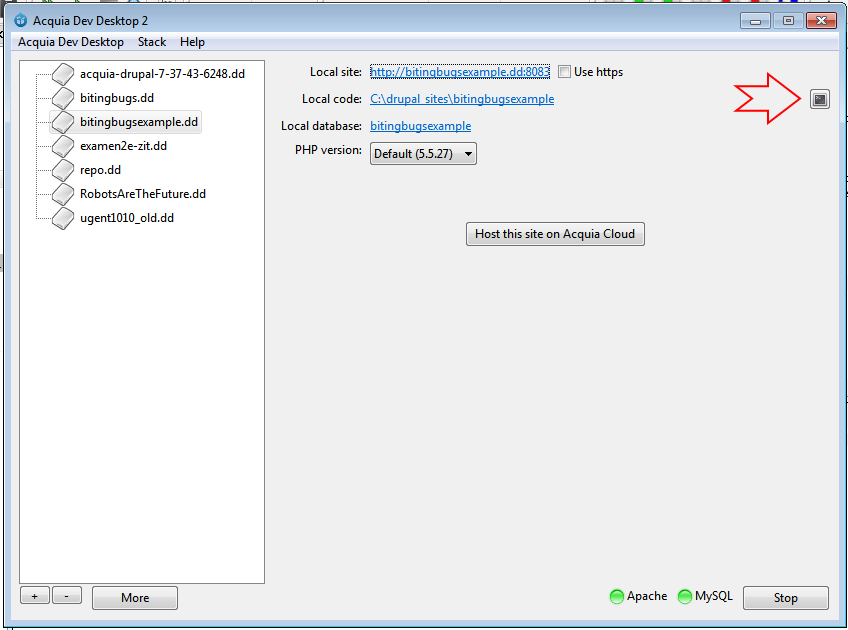
\includegraphics[width=\textwidth]{chapter8/console_window_button}
	\caption{Launch drush console button.}
	\label{fig:console_window_button}
\end{figure}

We will start by installing the \textbf{composer\_manager} module. Execute the following commands:

\begin{lstlisting}[language=bash]
	drush dl composer_manager  #downloads composer_manager module
	drush en composer_manager -y      #enables composer_manager module
\end{lstlisting}

\begin{figure}[H]
	\centering
	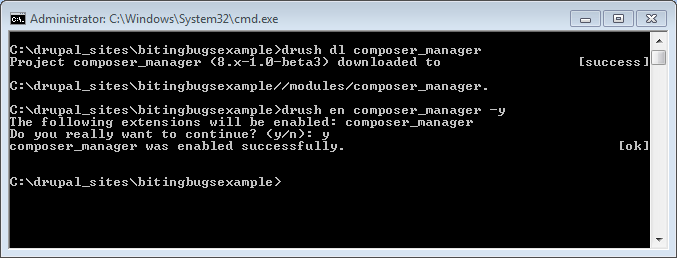
\includegraphics[width=\textwidth]{chapter8/drush_install_composer_manager}
	\caption{Downloading and enabling the composer\_manager module.}
	\label{fig:drush_install_composer_manager}
\end{figure}

The next step is initializing composer\_manager:

\begin{lstlisting}[language=bash]
drush composer-manager-init
\end{lstlisting}

The next step is installing the commerce module:

\begin{lstlisting}[language=bash]
drush dl commerce  #this generates an error!
\end{lstlisting}

The command above downloads the commerce module and tries to load the dependencies. The download is successful but the loading fails. This is because our drush installation can not find the \url{composer.phar} file. To solve this we are going to use absolute path values. On my computer the command is the following (you should change the path to match your Acquia Dev Desktop installation directory).

\begin{lstlisting}[language=bash]
cd core #change to the core folder
"C:\Program Files (x86)\DevDesktop\php5_6\php"
"C:\Program Files (x86)\DevDesktop\drush\composer.phar" drupal-update 
#perform a drupal update
\end{lstlisting}

Now we will enable the commerce module. Go to the bitingbugs site and go to: \textbf{Extend}. On the extend page there is a search box, search for \textit{commerce}. Select the \textbf{Commerce} module and click the \textbf{Install} button.

\begin{figure}[H]
	\centering
	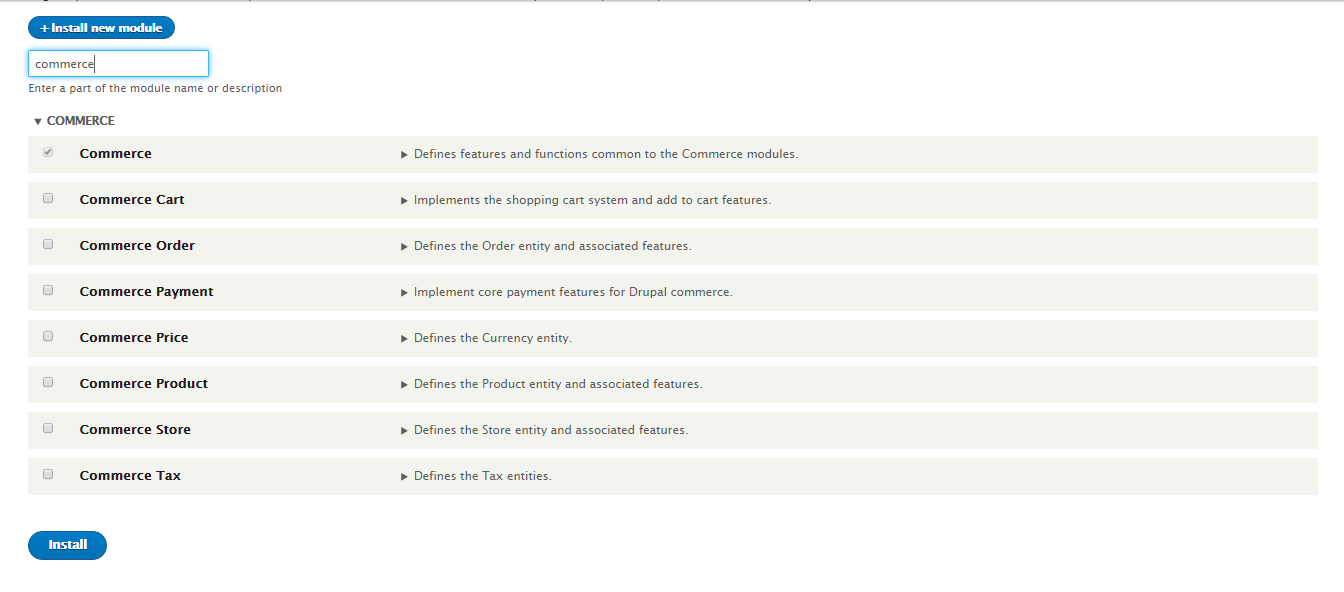
\includegraphics[width=\textwidth]{chapter8/enable_drupal_commerce_module}
	\caption{Enable Drupal commerce module.}
	\label{fig:enable_drupal_commerce_module}
\end{figure}

Do the same for the other commerce modules. You should enable them one by one because installing them all at once could lead to problems. After enabling the commerce module you should see a new link in the admin menu (Figure \ref{fig:commerce_in_admin_menu}).

\begin{figure}[H]
	\centering
	
\includegraphics[width=\textwidth]{chapter8/commerce_in_admin_menu}
	\caption{Commerce admin menu item.}
	\label{fig:commerce_in_admin_menu}
\end{figure}


\section{Adding a webstore to bitingbugs}





